\section{Molekulardynamik}
\label{md}

Ursprünglich mit dem Ziel der klassischen Simulation von Gasen und anderen Fluiden entwickelt, wurde die Molekulardynamik seither um die Fähigkeit zur Simulation von Festkörpern, organischen Molekülen und Reaktionen erweitert.
Dadurch findet sie Anwendung in Simulationen von Materialien und chemischen Stoffen bei beliebigen Temperaturen und Drücken, um deren Verhalten vorhersagen und auf reale Prozesse zurückführen zu können.

Nachfolgend möchte ich einen kurzen Überblick über die Formulierung molekulardynamischer Methoden geben (Abschnitt~\ref{mdformulation}) und im Anschluss auf die Unterschiede und Möglichkeiten der Kraftfelder eingehen (Abschnitt~\ref{mdforcefields}).

\subsection{Formulierung}
\label{mdformulation}

Molekulardynamik ist eine klassische Vielteilchenmethode, die jedem Teilchen des Systemes $X$ eine Masse $m$, eine Position $\vec r$, einen Impuls $\vec p$ und Kräfte entsprechend eines lokalen Kraftfeldes $\vec{F}(X)$ oder eventuellen Randbedingungen zuweist.
Entsprechend der Born-Oppenheimer-Näherung, nach der die Elektronen eines chemischen Systemes an ihre Atomkerne gebunden sind und schnell genug auf Änderungen des Systemes reagieren, genügt es, die Atome als Punktmassen an der Position ihres Atomkernes zu betrachten.
Elektronische und sonstige Interaktionen werden dann durch die verwendeten Kraftfelder beschrieben, die auf \todo{nochmal in Ruhe überdenken}Näherungen physikalischer Effekte basieren, um die Simulationszeit auf Kosten der Genauigkeit zu senken.

Der Systemzustand wird dann entweder entsprechend des gewählten Ensembles zeitlich integriert, oder hinsichtlich der Energie des Gesamt- oder eines Teilsystemes optimiert.
Dazu stehen Integratoren für das Mikrokanonischen Ensemble (NVE), das Kanonischen Ensemble (NVT) und das Großkanonischen Ensemble (NPT) ebenso zur Verfügung wie verschiedene Optimierungsmethoden, von denen hier die Konjugierte Gradienten-Methode vorgestellt werden soll.

\subsubsection{Mikrokanonisches Ensemble (NVE)}

Diese grundlegende Ensembleformulierung betrachtet die drei Größen Teilchenzahl $N$, Volumen $V$ und Systemenergie $E$ als zeitinvariant, um so vollkommen geschlossene Systeme zu untersuchen.

\begin{equation}
  N = \text{const.}
  \qquad
  V = \text{const.}
  \qquad
  E = \text{const.}
\end{equation}
Daraus ergibt ergeben sich die Bewegungsgleichungen für jedes Teilchen $i$, welche anschließend durch eine numerische Integrationsmethode, etwa dem Velocity-Verlet-Algorithmus, zeitlich integriert werden.

\begin{equation}
  \dot{\vec r_i} = \frac{\vec p_i}{m_i}
\end{equation}
\begin{equation}
  \dot{\vec p_i} = m \vec a_i = \vec F_i(X)
\end{equation}

\subsubsection{Kanonisches Ensemble (NVT)}

Aufbauend auf dem mikrokanonischen Ensemble tauscht das kanonische Ensemble zusätzlich Energie mit einem Wärmebad aus, so dass nicht mehr die Energie des Systems, sondern seine mittlere Temperatur $T$ konstant bleibt.

\begin{equation}
  N = \text{const.}
  \qquad
  V = \text{const.}
  \qquad
  T = \text{const.}
\end{equation}
Numerisch wird diese zusätzliche Randbedingung durch ein Thermostat ermöglicht, das die Teilchenenergien beeinflusst und so für eine Korrektur der mittleren Systemtemperatur in Richtung der Temperatur des Wärmebades sorgt.

Das \textbf{Berendsen-Thermostat}\cite{berendsen_molecular_1984} etwa skaliert die Teilchengeschwindigkeiten in Richtung des Mittelwertes der Maxwell-Boltzmann-Verteilung für die Zieltemperatur $T_\text{Ziel}$.
\begin{equation}
  \overline{E_{kin}} = \frac{1}{2} \overline{m v^2} = \frac{d}{2} k_B T_\text{Ziel}
\end{equation}
Anstatt einer harten Reskalierung wird für eine exponentielle Annäherung der Temperatur an $T_\text{Ziel}$ gesorgt, indem in jedem Zeitschritt nur ein Teil der Differenz in Abhängigkeit der Dämpfungszeit $\tau$ angeglichen wird.
\begin{equation}
  \vec v_i' = \vec v_i \cdot \sqrt{1 + \frac{\Delta t}{\tau} \left(\frac{T_\text{Ziel}}{T} - 1\right)}
\end{equation}
Dabei werden Fluktuationen in der Systemtemperatur unterdrückt und somit die Ergodizität verletzt, doch zeigt sich für große Systeme eine gute Annäherung an das kanonische Ensemble bei vertretbarer Rechenzeit.


%% Für kleine Systeme müssen jedoch Methoden benutzt werden, die das kanonische Ensemble bewahren.
%% Das \textbf{Andersen-Thermostat} beispielsweise tauscht über die Systemgrenzen hinweg Energie in Form von poissonverteilten Stößen mit virtuellen Teilchen aus und bewahrt so die Temperatur des Systems.
%% Zwar hat diese Vorgehensweise den Vorteil, mit einer geringen Anzahl an äußeren Einflüssen die Temperatur konstant zu halten, jedoch eignet es sich nur für die Betrachtung zeitgemittelter Größen, da lokale Energieeinträge in das System die Trajektorien einzelner Teilchen stören können.
%% In Zusammenhang mit der Untersuchung dynamischer Eigenschaften ist dieses Thermostat daher nicht zu empfehlen und sollte nur bei ausreichend großen Systemen Anwendung finden.

Die beste Alternative für kleine Systeme ist das \textbf{Nosé-Hoover-Thermostat}\cite{nose_unified_1984}\cite{hoover_canonical_1985}, das dem System einen zusätzlichen Freiheitsgrad $s$ hinzufügt, über den die Temperatur des Systems beeinflusst werden kann.
Durch die Bewahrung der Eigenschaften des kanonischen Ensembles hat sich das Nosé-Hoover-Thermostat als Standard-Thermostat in der Molekulardynamik durchgesetzt.
Der Einfluss auf die Teilchenenergien äußert sich in der Einführung einer zusätzlichen Reibungskraft entlang des Impulses jedes Teilchens:

\begin{equation}
  \dot{\vec p_i} = \vec{F_i} - s \vec{p_i}
\end{equation}
Der Reibungskoeffizient $s$ ändert sich in Abhängigkeit der Systemtemperatur, wobei er auch negative Werte annehmen und so Teilchen entlang ihrer Bewegungsrichtung beschleunigen kann.
Auch bei diesem Thermostat bestimmt der Faktor $\tau$, welcher mit der frei wählbaren Konstante $M$ multipliziert wird, das Zeitverhalten des Thermostates, also die mittlere Dauer zur Einstellung des thermodynamischen Gleichgewichtes.
$M$ enthält neben Einheitenfaktoren auch die virtuelle Masse des Wärmebades und wird üblicherweise so gewählt, dass $\tau$ unabhängig von der Masse und Größe des Systems ist.

\begin{equation}
  \dot s = \frac{1}{\tau M} \left(\sum_i{\frac{p_i^2}{2m_i}} - N d k_B T\right)
\end{equation}

\subsubsection{Großkanonisches Ensemble (NPT)}

Wird zusätzlich noch Verformungsarbeit vom oder am System verrichtet, ergibt sich das Großkanonische Ensemble, für das statt des Volumens der mittlere Druck des Systems konstant bleibt.

\begin{equation}
  N = \text{const.}
  \qquad
  p = \text{const.}
  \qquad
  T = \text{const.}
\end{equation}
Dies wird durch ein Barostat realisiert, das durch Skalierung des Simulationsraumes den mittleren Druck ähnlich zu den oben vorgestellten Thermostaten beeinflusst, sodass sich als Standard Nosé-Hoover-Barostate etabliert haben, gelegentlich aber auch Berendsen-Barostate verwendet werden.
Der Druck innerhalb des Systems wird dabei über die Virialgleichung ermittelt, die eigentlich für Gase gilt, aber auch für Flüssigkeiten und Feststoffe gute Ergebnisse liefert.

\begin{equation}
  P V = N k_B T + \frac{1}{d} \sum_{i=1}^N{\vec{r}_i \cdot \vec{F}_i}
\end{equation}

\todoline{Wenn Zeit bleibt: NPH betrachten}
\todoline{Wenn Zeit bleibt: Erforschung des Ensembles per Monte Carlo}

\subsubsection{Minimierung durch Konjugierte Gradienten (CG-Minimierung)}

\todoline{Hinweis von Jörg: beachte bitte, dass Prof. Hoffmann hier zuhause ist. Tiefergehende Kenntnisse können beim Vortrag nicht schaden}

\todoline{Betrachtung von Minimierungs-Algorithmen, etwa auch Simulated Annealing}
Für die Strukturoptimierung mit molekulardynamischen Methoden werden Algorithmen zur Energieminimierung genutzt, wie die populäre Konjugierte-Gradienten-Methode (CG, Conjugated Gradients), mit denen im Idealfall das globale Minimum der Systemenergie gesucht wird.
\todo{0K}Bei der CG-Methode wird der Zustandsraum von einem Startzustand $\vec X_0$ aus entlang des Gradienten der Energie $\nabla E(X)$ in Richtung des Minimums abgeschritten, wobei über die Schrittweite $\alpha$ das Konvergenzverhalten beeinflusst werden kann.
\begin{figure}
  \centering
  \def\svgwidth{0.5\textwidth}
  \input{img/cg-gradient.pdf_tex}
  \caption[Minimierung durch Konjugierte Gradienten]{
    Minimierung durch konjugierte Gradienten:\\
    a) Optimale Schrittweite\\
    b) Kleine Schrittweite $\Rightarrow$ viele unnötige Schritte\\
    c) Große Schrittweite $\Rightarrow$ langsames Konvergenzverhalten
  }
  \label{fig:cg-gradient}
\end{figure}
\begin{equation}
  \vec X_i = \vec X_{i-1} - \alpha \nabla E(\vec X_{i-1})
\end{equation}
Als Abbruchkriterien stehen je nach Verhalten des Systems währen der Optimierung die Differenz zwischen zwei Schritten ($|\vec X_i - \vec X_{i-1}| < X_\text{tol}$), die maximale Änderung eines Vektorelementes ($\max_k{|X_{i,k} - X_{i-1,k}|} < X_\text{tol}$),
die Stärke des Gradienten ($|\nabla E(\vec X_{i-1})| < E_\text{tol}$), eine Anzahl an Zeitschritten ($i > i_\text{tol}$) oder eine Kombination daraus zur Verfügung.

Eine Optimierung durch minimierte Gradienten ist für eine große Zahl an Freiheitsgraden zwar schnell\todo{verglichen womit?}, stößt aber an Grenzen bei der Minimierung allgemeiner nichtlinearer Funktionen, weshalb Variationen der CG-Methode mit besserem Konvergenzverhalten entwickelt wurden.
Einerseits kann der Optimierungsschritt durch eine Minimierung entlang der Richtung des Gradienten ersetzt werden:
\begin{gather}
  \min_\alpha f(X_i+\alpha \vec s_i) \rightarrow \alpha_i \\
  \vec X_i = \vec X_{i-1} - \alpha_i \vec s_i
\end{gather}
Andererseits steht die Manipulation der Schrittrichtung in Abhängigkeit vorheriger Schritte zur Verfügung.
In der populären MD-Bibliothek LAMMPS wird etwa die Polak-Ribière-Variante dieser Methode genutzt:
\begin{equation}
  \vec s_i = \Delta \vec X_i + \beta_i \vec s_{i-1}
\end{equation}
\begin{equation}
  \beta_i = \max \left(0, \frac{\Delta \vec X_i \cdot \left(\Delta \vec X_i - \Delta \vec X_{i-1}\right)}{\Delta \vec X_{i-1} \cdot \Delta \vec X_{i-1}}\right) \text{~(Polak-Ribière)}
\end{equation}
Es existieren noch weitere gleichwertige Methoden mit anderen Zielsetzungen und Formulierungen.\todo{Das ist mal schwammig. Wenigstens Beispiele bringen, besser noch Referenzen}
Diese Anpassungen verbessern einerseits das erwartete Konvergenzverhalten, andererseits stabilisieren sie den Optimierungsalgorithmus gegenüber Nichtlinearitäten und Unstetigkeiten.

%% \subsubsection{Weitere Minimierungsmethoden}

%% Es stehen noch weitere Minimierungsalgorithmen zur Verfügung, wie beispielsweise die Klasse der Newton-Verfahren.
%% Obwohl diese auf dem Papier schneller konvergieren, sind für jeden Iterationsschritt durch die Berechnung der Hesse-Matrix mehr Rechenoperationen notwendig, so dass reale Berechnungszeit und Speicherverbrauch gegenüber CG-Methoden oft im Nachteil sind.

%% separate file for force fields to avoid having to scroll down
\subsection{Kraftfelder}
\label{mdforcefields}

Zentrales Element molekulardynamischer Methoden sind Kraftfelder~$\vec F(X)$, auch Potentiale~$V(X)$ genannt, welche die Interaktionen der simulierten Teilchen beschreiben.
Für verschiedene Materialien existieren spezielle Potentialformulierungen, die für unterschiedliche Elemente wiederum eigene Potentialparametrisierungen in Form von Potentialdateien zur Verfügung stellen.
Im Folgenden soll eine Auswahl dieser Potentialformulierungen kurz in ihrer Funktionsweise vorgestellt werden.

\subsubsection{Paar-Potentiale}

Das einfachste MD-Potential ist das Paarpotential, welches Interaktionen zwischen jeweils zwei benachbarten Atomen modelliert.
Damit vereinfacht sich die Energie des Gesamtsystems auf Summen des Potentiales $V$ über alle Paare von Atomen in Abhängigkeit ihres Abstandes $r_ij$:
\begin{equation}
  \label{eq:pairforce}
  \vec F_{ij}(r_{ij}) = \vec\nabla V(r_{ij})
\end{equation}
\begin{equation}
  \label{eq:pairenergy}
  E = \sum_i\sum_{j \neq i}{V(r_{ij})}
\end{equation}

Stellvertretend steht das Lennard-Jones-Potential zur Darstellung von allgemeinen Fluiden:
\begin{equation}
  \label{eq:lennardjones}
  V_\text{LJ}(r_{ij}) = 4 \epsilon \left[\left(\frac{\sigma}{r_{ij}}\right)^{12} - \left(\frac{\sigma}{r_{ij}}\right)^{6}\right]
\end{equation}

Weitere Paarpotentiale wie etwa das mit dem Lennard-Jones-Potential verwandte Bucking\-ham-Potential nehmen aufgrund unterschiedlicher Anwendungsgebiete andere Formen an (Abbildung~\ref{fig:mdpairpotentials}).
Allen Paar-Potentialen ist gemein, eine rein radiale Abhängigkeit $V(r_ij)$ zu besitzen, die oftmals einen charakteristischen Bindungsabstand in Abhängigkeit der Parameter bildet, welcher sich als Minimum in den Potentialen äußert.
Unterhalb dieses Radius' dominiert ein repulsiver Term, wo hingegen oberhalb davon ein leicht attraktiver Term vorherrscht, der sich für große Radien einem konstanten Wert annähert und deshalb mit einem Cutoff-Radius $r_\text{cut}$ versehen ist.


\begin{figure}
  \centering
  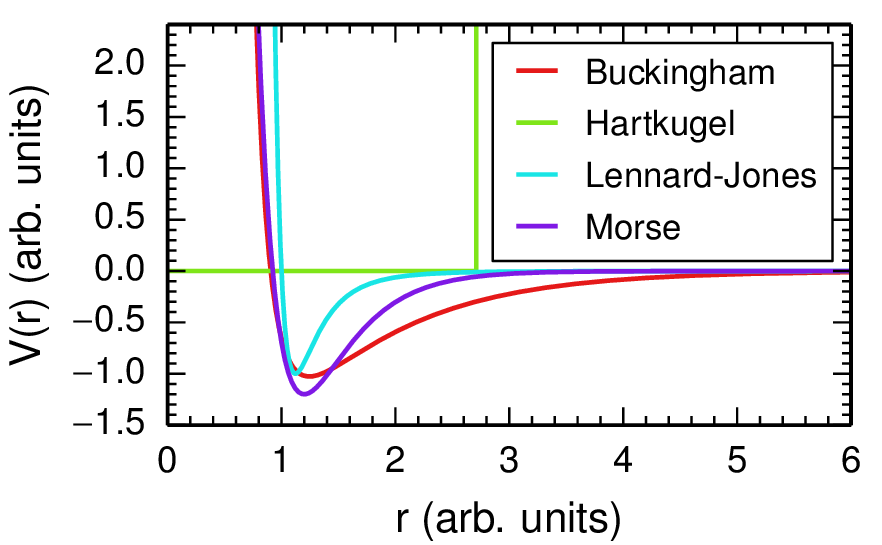
\includegraphics[width=0.5\textwidth]{mdpotplot}
  \caption{Auswahl einfacher molekulardynamischer Paarpotentiale}
  \label{fig:mdpairpotentials}
\end{figure}

\todo{Beleg, Zitat, Nachweis}Zwar zeigen Paarpotentiale gute thermodynamische Eigenschaften bei geringem Rechenaufwand, doch können sie aufgrund ihrer simplen Formulierung keine atomistischen Strukturen verlässlich vorhersagen.

\subsubsection{N-Teilchen-Potentiale}

N-Teilchen-Potentiale erweitern Paarpotentiale um weitere Terme, die von der Position einer festen Anzahl an Teilchen abhängen.
Damit können beispielsweise Winkel- und Torsionsabhängigkeiten wiedergegeben werden.

\begin{equation}
  \label{eq:nbody-energy}
  E = \sum_i\sum_{j \neq i}{V_2\left(r_{ij}\right)} + \sum_i\sum_{j \neq i}\sum_{\substack{k \neq i \\ k \neq j}}{V_3\left(r_{ij}, r_{ik}, \theta_{ijk}\right)} + \dots
\end{equation}

Obwohl sich mit N-Teilchen-Potentialen komplexere Systeme betrachten lassen, zeigen sie die gleichen Schwachstellen wie Paarpotentiale, benötigen aber eine größere Anzahl an Parametern,
Zwar gibt es erfolgreiche Anwendungen für Biomoleküle (\todo{CHARMM} \todo{GROMACS} \todo{AMBER}), die allerdings aufgrund ihrer Spezialisierung nicht auf andere Stoffsysteme wie Festkörper oder Oberflächen übertragbar sind.

\subsubsection{Embedded Atom Model}

Das Embedded Atom Model (EAM) besteht aus einem Paarpotential $V_{\alpha\beta}(r_{ij})$ für jedes Atom $i$ sowie einer Einbettungsfunktion $F_\alpha$, welche die Energie des Atomes in Abhängigkeit der angenäherten lokalen Elektronendichte $\rho_\beta(r_{ij})$ modelliert\cite{daw_embedded-atom_1984}.
\begin{equation}
  \label{eq:eam-energy}
  E = \sum_i\left[F_\alpha\left(\sum_{j\neq i}{\rho_\beta\left(r_{ij}\right)}\right) + \frac{1}{2}\sum_{j\neq i}{V_{\alpha\beta}\left(r_{ij}\right)}\right]
\end{equation}
So lassen sich metallische Bulksysteme und Oberflächen simulieren, für die $\alpha$ und $\beta$ verschiedene Spezies darstellen, doch führt die Formulierung für andere Systeme zwangsläufig zur Bildung von Clustern\todo{ggfs. erläutern oder durch Zitat belegen}.
Für eine Vielzahl an Metallen und Legierungen findet man in Potentialdatenbanken fertige Parametrisierungen\cite{becker_interatomic_2014}, von denen viele zusätzlich zu den strukturellen auch thermodynamische Eigenschaften recht gut modellieren (Abschnitt~\ref{goldthermo}).

%% \subsubsection{Modified Embedded Atom Model}

Für Metalloxide und weitere Mischsysteme existiert eine Erweiterung in Form des Modified Embedded Atom Models\cite{baskes_modified_1992}, dem eine umfangreichere Formulierung der lokalen Elektronendichten zugrunde liegt.

%% Als Erweiterung des EAM-Potentials wurden MEAM-Potentiale entwickelt, die neben Metallen und Legierungen auch Metalloxide und andere Mischsysteme ermöglichen sollen\cite{baskes_modified_1992}.
%% Sie basieren auf der gleichen Funktionsweise, stellen die Einbettungsenergie aber in Abhängigkeit einer umfangreicheren Formulierung der lokalen Elektronendichte dar.
%% Aufgrund der umfangreichen Formulierung soll auf die ursprüngliche Publikation von Baskes\cite{baskes_modified_1992} verwiesen werden.

%% \begin{equation}
%%   \label{eq:meam-energy}
%%   E = \sum_i\left[F_\alpha\left(\bar{\rho_i}\right) + \frac{1}{2}\sum_{j\neq i}{V_{ij}\left(r_{ij}\right)}\right]
%% \end{equation}

\subsubsection{Reactive Force Fields}

Reaktive Kraftfelder (Reactive Force Fields, ReaxFF) wurden von \textsc{van Duin et al.}\cite{van_duin_reaxff:_2001} 2001 mit dem Ziel entwickelt, Reaktionen zwischen Molekülen mit molekulardynamischen Methoden beschreiben zu können.
Mangels expliziter Beschreibung der involvierten Elektronen war die Beschreibung von Bindungen zuvor nur mit Elektronenstrukturrechnungen möglich, denen aber eine obere Grenze von wenigen hundert Atomen gesetzt ist.
Durch Beschreibung der Über- und Unterkoordination der Atome innerhalb ihrer Nachbarschaft, zusätzlich zum Ladungsaustausch zwischen den Atomen, Van-der-Waals- und elektrostatischen Kräften, lassen sich mit der ReaxFF-Formulierung Bindungen während der Simulation dynamisch formen und lösen, wodurch die Simulation von Reaktionen ermöglicht wird.
Gleichung~\ref{eq:reaxformulation} und Tabelle~\ref{tab:reaxenergies} geben einen kurzen Überblick über die Summanden der Gesamtenergie, von denen die meisten Terme über die Bindungsordnung berechnet werden, welche sich aus Beiträgen für $\sigma$-, $\pi$- und Doppel-$\pi$-Bindungen aus dem Bindungsabstand zusammen setzt.
Darüber hinaus werden einige Terme in der Nähe des Cutoff-Abstands sowie an Koordinations-Übergängen auf 0 gesenkt, um Diskontinuitäten zu vermeiden und einen fließenden Übergang zwischen Bindungszuständen zu ermöglichen.

\begin{align}
  \label{eq:reaxformulation}
  E_\text{system} =~& E_\text{bond} + E_\text{lp} + E_\text{over} + E_\text{under} + E_\text{val} + E_\text{pen} + E_\text{coa} + E_\text{C2} \\
  \nonumber  & + E_\text{tors} + E_\text{conj} + E_\text{H-bond} + E_\text{vdWaals} + E_\text{Coulomb}
\end{align}

\begin{table}
  \oddrowcolors
  \caption[Summanden der ReaxFF-Gesamtenergie]{
    Erläuterung der Summanden der ReaxFF-Gesamtenergie aus Gleichung~\ref{eq:reaxformulation}\cite{van_duin_reaxff:_2001}
  }
  \label{tab:reaxenergies}
  \begin{tabularx}{\textwidth}{|llX|}
    \hline
    \textbf{Term}      & \textbf{Beitrag}            & \textbf{Kommentar}                            \\
    \hline
    $E_\text{bond}$    & Bindungsenergien            & Berechnung über Bindungsordnung               \\
    $E_\text{lp}$      & freie Elektronenpaare       & über Bindungsordnungssumme am Atomzentrum     \\
    $E_\text{over}$    & Überkoordinationen          & unter Ausschluss freier Elektronenpaare       \\
    $E_\text{under}$   & Unterkoordinationen         & nur bei unterkoordinierten $\pi$-Bindungen    \\
    $E_\text{val}$     & Bindungswinkel              & Optimum abhängig von Elektronenkonfiguration  \\
    $E_\text{pen}$     & Strafenergien               & Fehlerkorrektur bei Winkeln mit Doppelbindung \\
    $E_\text{coa}$     & Drei-Teilchen-Konjugationen & Stabilisierung von NO$_2$-Gruppen             \\
    $E_\text{C2}$      & Dreifachbindungskorrektur   & Stabilisierung der Dreifachbindung von C$_2$  \\
    $E_\text{tors}$    & Torsionsbarrieren           &                                               \\
    $E_\text{conj}$    & Vier-Teilchen-Konjugationen & Konjugation bei Kohlenwasserstoffen           \\
    $E_\text{H-bond}$  & Wasserstoffbrücken          &                                               \\
    $E_\text{vdWaals}$ & Van-der-Waals-Kräfte        &                                               \\
    $E_\text{Coulomb}$ & Coulomb-Kräfte              &                                               \\
    \hline
  \end{tabularx}
\end{table}

Aus den Termen des ReaxFF-Potentials geht hervor, dass es ursprünglich für Reaktionen von organischen Molekülen entwickelt wurde, doch hat es sich als vielseitig genug herausgestellt, auch eine Vielzahl anderer Materialien wie Kristalle und nichtorganische Verbindungen simulieren zu können.
Die einzige Abhängigkeit besteht zum Trainingssatz, also den Test-Strukturen, an deren Werte die Parametrisierung des Reax-Kraftfeldes angepasst wurde.
So kann die Parametrisierung in der Regel nur die Strukturen und Materialien zuverlässig wiedergeben, für die sie ursprünglich erstellt wurde.
Für darüber hinaus gehende Anwendungen ist \todo{in der Regel}eine aufwendige Anpassung der Parametersätze mittels geeigneter Trainingsstrukturen erforderlich.\todo{Zitat?}

In den letzten fünf Jahren haben Reactive Force Fields jedoch an Aufmerksamkeit gewonnen, so dass die Zahl verfügbarer spezialisierter Parametrisierungen stetig zunimmt.
Es gibt auch Bestrebungen, sich ergänzende ReaxFF-Parametrisierungen zu kombinieren und somit mit einer Parametrisierung eine große Zahl von Zielsystemen betrachten zu können.
Besonders in kommerzieller MD-Software\cite{biovia_materials_2014} versucht man so, dem Nutzer ein umfassendes Paket für die Simulation beliebiger Strukturen zu präsentieren, ohne ihm aber die Grenzen der Vorhersagekraft des Parametersatzes erkenntlich zu machen.


\subsection{Verfügbare Software}

Für molekulardynamische Simulationen stehen sowohl kommerzielle als auch freie Softwarepakete zur Verfügung, die jeweils eigene Parametersätze mitbringen.
In LAMMPS lassen sich zudem auch externe Parametersätze einbinden, wodurch die Betrachtung neuer Problemstellungen erleichtert wird.
Weiterhin unterscheiden sich die Programme in ihrer Nutzerfreundlichkeit (Kommandozeile oder grafische Oberfläche) und der Möglichkeit, sie als Bibliothek in eigene Programme einzubinden.
Tabelle~\ref{tab:mdsoftware} stellt ausgewählte Vertreter moderner Molekulardynamiksoftware dar.

\begin{table}
  \oddrowcolors
  \caption[Verfügbare Molekulardynamik-Software]{
    Verfügbare Molekulardynamik-Software
  }
  \label{tab:mdsoftware}
  \begin{tabularx}{\textwidth}{|llX|}
    \hline
    \textbf{Paket}                                                               & \textbf{Autor/Rechteinhaber}   & \textbf{Beschränkungen \& Kommentare}                            \\
    \hline
    LAMMPS\cite{plimpton_lammps_2014,plimpton_fast_1995}                         & Sandia                   & quelloffen, Kommandozeile, Bibliothek, eigene Potentiale möglich \\
    Materials Studio\cite{biovia_materials_2014}                                 & BIOVIA                   & Grafische Oberfläche, lizenzpflichtig                            \\
    AMBER\cite{case_amber_2014,case_amber_2005}                                  & University of California & Biomoleküle, lizenzpflichtig                                     \\
    CHARMM\cite{brooks_charmm_2014,brooks_charmm:_1983,brooks_charmm:_2009}      & BIOVIA                   & Proteine, lizenzpflichtig                                        \\
    GROMACS\cite{lindahl_gromacs_2014,berendsen_gromacs:_1995,hess_gromacs_2008} & Uppsala University       & Biomoleküle, quelloffen                                          \\
    \hline
  \end{tabularx}
\end{table}
